\documentclass[a4paper]{article}
\usepackage[utf8]{inputenc}
\usepackage[14pt]{extsizes}
\usepackage[russian]{babel}
\usepackage{setspace,amsmath}
\usepackage{lscape}
\usepackage[left=20mm, top=20mm, right=20mm, bottom=20mm]{geometry}
\setlength{\parindent}{12,5mm}
\linespread{1.15}
\usepackage{fontspec} 
\defaultfontfeatures{Ligatures={TeX},Renderer=Basic} 
\setmainfont[Ligatures={TeX,Historic}]{Times New Roman}
\usepackage{multirow}

\usepackage{graphicx}
\graphicspath{{pictures/}}
\DeclareGraphicsExtensions{.pdf,.png,.jpg}

\begin{document}
    \begin{titlepage}
    \large{
        \begin{center}
            Белорусский Национальный Технический Университет\\
            Факультет Транспортных Коммуникаций\\
            Кафедра <<Геодезия и аэрокосмические геотехнологии>>\\
            ~\\
            ~\\
            ~\\
            ~\\
            ~\\
            ~\\
            Отчет\\
            по учебно-геодезической практике\\
            (Высшая геодезия)\\
            ~\\
            ~\\
            ~\\
            ~\\
            ~\\
        \end{center}
        
        \begin{flushright}
            Выполнил: Бригада №4\\
            Греченков Т.А.\\
            Гречный К.М.\\
            Лабудев Н.А.\\
            Прудников М.К.\\
            Рогожников И.А.\\
            Проверил ст. преподаватель\\
            Будо А.Ю.
            ~\\
            ~\\
            ~\\
            \begin{center}
                Минск,2021
            \end{center}
            
        \end{flushright}
    }
\end{titlepage}

\begin{newpage} % Оглавление
\large{
    \begin{center}
        \textbf{Оглавление}
    \end{center}
    ~\\
    \begin{center}
        Полигонометрия 4 класса..................................................................2\\
        Нивелирование III класса..................................................................8\\
        Спутниковые измерения методом быстрой статики.....................11\\
        Приложение А. Технические характристики приборов...............17\\
        Приложение Б. Поверки Электронного нивелира DL-202...........26\\
        Приложение В. Поверки элетронного теодолита DT-2A..............28\\
        Приложение Г. Абрисы пунктов.....................................................32\\
        Приложение Д. Ведомость круговых приёмов..............................37\\
        Приложение Е. Журнал нивелирования III класса........................50\\
        Приложение Ж. Ведомость оцнки точности положения\;\;\;\;\;\;\;\;\;\;\;\;\;\;\;\;\\
        пунктов...............................................................................................51\\
        Приложение З. Каталог пунктов ПВО............................................52\\
        Приложение И. Схема сети полигонометрии................................53\\
    \end{center}
}
\end{newpage}

\begin{newpage}

    \large{
        \begin{center}
            \textbf{Полигонометрия 4 класса}
        \end{center}
        
        \par Полигонометрические сети 4 класса, 1 и 2 разрядов создаются в виде отдельных ходов или различных систем ходов. Полигонометрии 4 класса для крупномасштабных съемок выполняется с пониженной точностью.
        \par Отдельный ход полигонометрии должен опираться на 2 исходных пункта. На исходных пунктах необходимо измерять примычные углы. В исключительных случаях при отсутствии между исходными пунктами видимости с земли допускается:
        \par - проложение хода полигонометрии, опирающегося на 2 исходных пункта, без угловой привязки на одном из них. Для контроля угловых измерений используются дирекционные углы на ориентирные пункты государственной геодезической сети.
        \par - проложение замкнутого хода полигонометрии 1, 2 разрядов опирающегося на один исходный пункт, при условии передачи или измерения с точек хода двух дирекционных углов с точностью 5 − 7” на две смежные стороны по возможности в слабом месте (середине) хода;
        \par - координатная привязка к пунктам геодезической сети. При этом для контроля угловых измерений в целях обнаружения грубых ошибок измерений используются дирекционные углы на ориентирные пункты, полученные из астрономических измерений.
        \par\textit{Проложение висячих ходов не допускается.}
        \par При построении полигонометрических сетей 4 класса, 1 и 2 разрядов должны соблюдаться требования, приведенные, таблице 1.
        \\
        \\
        \\
        \\
        Таблица 1 – Показатели полигонометри
        \begin{center}
            \normalsize{
                \begin{tabular}{|p{280pt}|c|c|c|}
                    \hline
                    Показатели & 4 класс & 1 разряд & 2 разряд\\
                    \hline
                    Предельная длина хода, км: &  &  &\\
                    \hline
                    отдельного & 15 & 5 & 3\\
                    \hline
                    между исходной и узловой точкой & 10 & 3 & 2\\
                    \hline
                    между узловыми точками & 7 & 2 & 1.5\\
                    \hline
                    Предельный параметр полигона, км & 30 & 15 & 9\\
                    \hline
                    Длины сторон хода, км: &  &  &\\
                    \hline
                    наибольшая & 2.00 & 0.80 & 0.35\\
                    \hline
                    наименьшая & 0.25 & 0.12 & 0.08\\
                    \hline
                    средняя расчетная & 0.50 & 0.30 & 0.20\\
                    \hline
                    Число сторон в ходе, не более & 15 & 15 & 15\\
                    \hline
                    Относительная погрешность хода, не более & 1:25000 & 1:10000 & 1:5000\\
                    \hline
                    Средняя квадратическая погрешность измерения угла (по невязкам в ходах, и полигонах) угловые секунды, не более & 3 & 5 & 10\\
                    \hline
                    Угловая невязка хода или полигона, не более & $5\sqrt{n}$ & $10\sqrt{n}$  & $20\sqrt{n}$\\
                    \hline
                \end{tabular}
            }
        \end{center}
        
        \par Расстояние между пунктами параллельных полигонометрических ходов данного класса (разряда), по длине близких к предельным, должно быть не менее:
        \par - в полигонометрии 4 класса - 2,5 км;
        \par - в полигонометрии 1 разряда - 1,5 км.
        \par При меньших расстояниях ближайшие пункты должны быть связаны ходом полигонометрии данного класса (разряда). Если пункты хода полигонометрии 1 разряда отстоят мене чем на 1,5 км от пунктов параллельного хода полигонометрии 4 класса, то между этими ходами должна быть осуществлена связь приложением хода 1 разряда.
        \par При проложении полигонометрических ходов 1 и 2 разрядов больше указанной в таблице 1 протяженности необходимо определять дирекционные углы сторон хода с точностью 5−7” не реже чем через 15 сторон и не реже чем через 3 км.
        \par На все закрепленные точки полигонометрических ходов должны быть переданы отметки нивелированием IV класса или техническим нивелированием. В горной местности при обеспечении съемок с сечением рельефа через 2 и 5 м допускается определение высот точек полигонометрических ходов тригонометрическим нивелированием.
        \par Измерение углов на пунктах полигонометрии производится способом измерения отдельного угла или способом круговых приемов, как правило, по трехштативной системе оптическими теодолитами Т1, Т2, Т5 и другими, им равноточными, с точностью центрирования 1 мм.
        \par При измерениях способом отдельного угла алидада вращают только по ходу часовой стрелки или только против хода часовой стрелки.
        \par При измерениях круговыми приемами в первом полуприеме алидаду вращают по ходу часовой стрелки, а во втором - в обратном направлении.
        \par Число приемов, в зависимости от класса (разряда) полигонометрии и типа применяемого прибора, приведено в Таблице 2\\
        
        Таблица 2 – Число приемов в полигонометрии
        \begin{center}
            \begin{tabular}{|c|c|c|c|}
                \hline
                \multirow{2}{*}{Типы прибора} & \multicolumn{3}{c|}{Число приёмов в полигонометрии}\\
                \cline{2-4}
                & 4 класс & 1 разряд & 2 разряд\\
                \hline
                Т1 и ему равноточный & 4 & - & -\\
                \hline
                Т2 и ему равноточные & 6 & 2 & 2\\
                \hline
                Т5 и ему равноточные  & - & 3 & 2\\
                \hline
            \end{tabular}
        \end{center}
        
        \par При переходе от одного приема к другому лимб переставляется на угол $180/n + \sigma$, где n - число приёмов, а $\sigma = 10′$ или $5′$.\\
        
        Таблица 3 – Допуски для приборов
        \begin{center}
            \normalsize{
                \begin{tabular}{|p{280pt}|c|c|}
                    \hline
                    \multirow{2}{*}{Основные элементы угловых измерений} & \multicolumn{2}{c|}{Допуски для приборов}\\
                    \cline{2-3}
                    & Типа Т2 & Типа Т5\\
                    \hline
                    Расхождения в полуприёмах & 8′′ & 0,2′\\
                    \hline
                    Расхождения в приёмах & 8′′ & 0,2′\\
                    \hline
                    Колебание значения 2С в приёмах & 12′′ & –\\
                    \hline
                    Колебание между повторными наблюдениями начального направления в начале и конце полуприёма & 8′′ & 0,2′\\
                    \hline
                    Колебание направлений в отдельных приёмах, приведенных к общему нулю & 8′′ & 0,2′\\
                    \hline
                \end{tabular}
            }
        \end{center}
        
        \par Если разность зенитных расстоянии на два измеряемых направления более 20°, допуски расхождений между значениями одного и того же угла, полученного из двух полуприемов, увеличиваются в 1,5 раза. При наличии в группе измерений отдельных приемов или углов, результаты которых не удовлетворяют установленным допускам, последние повторяются на тех же установках лимба. Если среднее значение угла (направления), полученное из основного и повторного измерений, удовлетворяет установленным допускам, то оно принимается в дальнейшую обработку. В противном случае основной прием вычеркивается и в обработку принимается повторный.
        \par Расхождения между значениями измеренного и исходного угла на примычном пункте в полигонометрии не должны превышать:
        \par - 4 класса - 6′′,
        \par - 1 разряда - 10′′,
        \par - 2 разряда - 20′′,
        \par Если расхождения будут более указанного допуска, то определяется третье исходное направление, по которому следует произвести соответствующий контроль.
        \par Теодолит и визирные цели должны устанавливаться над центрами с точностью 1 мм с помощью оптического центрира.
        \par При наблюдениях со столиков сигналов или на визирные цели сигналов (пирамид) должны определяться элементы приведения графическим способом дважды (до начала наблюдений и после).
        \par Угловые и линейные измерения рекомендуется производить одновременно. При этом полевая обработка материалов измерений и контрольные вычисления должны, как правило, производиться исполнителем.
        \par Линии в полигонометрии 4 класса, 1 и 2 разрядов измеряются светодальномерами, радиодальномерами, а в отдельных случаях - базисными приборами БП-2 и БП-3 или тахеометром ТЭ и другими приборами и методами, обеспечивающими точность, соответствующую классу или разряда полигонометрии. В полигонометрии 1 и 2 разряда для измерения могут быть использованы длиномер типа АД-1 и параллактический метод, в полигонометрии 2 разряда, кроме того, - редукционные тахеометры ТД (ГОСТ 10812-74) и Редта-002. Приборы и оборудование, фиксирующие концы линии при ее измерении, должны устанавливаться над центрами с точностью 1 мм.
        \par Измерение линий светодальномерами других типов и радиодальномерами производится методами и числом приемов в зависимости от конкретного типа дальномера согласно действующим инструкциям по их применению.
        \par Для измерения параллактических углов применяются теодолиты Т2 и ему равноточные. Параллактические углы измеряются четырьмя приемами; средняя квадратическая погрешность угла, вычисленная по сходимости приемов, должна быть не более 1,5”. Расхождения значений из разных приемов не должны превышать 3 в противном случае делаются дополнительные измерения. Измерение параллактических углов производится на одной части лимба, точность нанесения штрихов которой тщательно исследуется. В случае, если погрешности в положении штрихов превышают 1 в измеренные параллактические углы следует вводить поправки. Редукционными тахеометрами ТП и Редта-002 линии измеряются в прямом и обратном направлениях. Линии длиннее 170 м измеряются по частям, при этом отклонение промежуточных точек от створа линии не должно превышать 0,4 м. Измерение линии в одном направлении выполняется двумя приемами. Прием состоит из двукратного совмещения штрихов на рейке и двукратного отсчета: первый отсчет при вращении дистанционного барабана по ходу часовой стрелки (вправо), второй - при вращении против хода часовой стрелки (влево).
        \par Предельное расхождение результатов измерений линии должно быть не более:
        \par - между приемами - 1:3000.
        \par - между прямым и обратным измерениями - 1:5000.
        \par В измеренные расстояния вводятся поправки за величину постоянного слагаемого и коэффициент дальномера, если последние не равны соответственно 0 и 100. Постоянное слагаемое и коэффициент дальномера определяются на полевом компараторе перед началом и после окончания работ, а также, если тахеометр подвергся удару или сильной тряске. Для измерения сторон полигонометрии 1 и 2 разрядов на застроенной территории может быть применен короткобазисный параллактический метод. При измерении этим методом применяются оптические теодолиты Т2 и ему равноточные, 2-метровые рейки «Бала» и визирные марки.
    }
    
\end{newpage}

\begin{newpage}

    \large{
        \begin{center}
            \textbf{Нивелирование III класса}
        \end{center}
        
        \par Способ нивелирования III класса зависит от применяемых нивелиров. Предпочтение отдают нивелирам с самоустанавливающейся линией визирования (с компенсатором).
        \par Нивелиры и рейки исследуют и поверяют с целью установления их пригодности для нивелирования III класса, приведения в рабочее состояние и определения постоянных. Нивелирование III класса производят в прямом и обратном направлениях ”способом средней нити”или ”способом совмещения”.
        \par Поскольку в современных нивелирах сетка зрительной трубы не содержит нитей, правильнее было бы назвать «способ среднего штриха» или «способ наведения»
        \par Необходимая точность нивелирования может быть достигнута только в том случае, если обеспечено верное взаиморасположение основных осей нивелира. Для контроля предъявляемых к прибору требований в начале и периодически в ходе работ выполняют поверки нивелира. Основными поверками являются следующие:
        \par 1. Ось круглого уровня должна быть параллельна оси вращения нивелира.
        \par 2. Вертикальная нить сетки должна совпадать с отвесом (быть параллельна вертикальной оси вращения нивелира).
        \par 3. Поверка главного условия.
        \par После выполнения поверок можно приступать к работе.
        \par Порядок наблюдений на станции следующий:
        \par ∙ отсчет по черной стороне (основной шкале) задней рейки;
        \par ∙ отсчет по черной стороне (основной шкале) передней рейки;
        \par ∙ отсчет по красной стороне (дополнительной шкале) передней реки;
        \par ∙ отсчет по красной стороне (дополнительной шкале) задней рейки.
        \par Нивелирование выполняют участками в 20-30 км. Переход от нивелирования в прямом направлении к нивелированию в обратном направлении делают только на постоянных знаках. При этом рейки меняют местами.
        \par Нормальная длина луча визирования - 75 м. При отсутствии колебаний изображения реек и увеличения трубы не менее 35 длину луча разрешается увеличивать до 100 м.
        \par Расстояния от нивелира до реек измеряют тонким тросом, просмоленной бечевой или дальномером; неравенство расстояний на станции допускают не более 2 м, а их накопление по секции - не более 5 м.
        \par Высота луча визирования над подстилающей поверхностью должна быть не менее 0,3 м.
        \par Нивелирование выполняют при хорошей видимости, отчетливых и спокойных изображениях реек. В солнечные дни не следует нивелировать в периоды, близкие к восходу и заходу солнца.
        \par При работе на станции нивелир с уровнем защищают от солнечных лучей зонтом.
        \par Рейки устанавливают по уровню на костыли или башмаки. В местах установки башмаков предварительно снимают дерн. Для удобства рекомендуется пользоваться не менее чем тремя костылями или башмаками.
        \par При нивелировании способом «средней нити» необходимо соблюдать следующие допуски.
        \par Отсчет по средней нити по черной стороне каждой рейки не должен расходиться более чем на 3 мм с соответствующей полу-суммой отсчетов по дальномерным нитям.
        \par Расхождение между значениями превышения, полученными по черным и красным сторонам реек, не должно быть более 3 мм с учетом разности высот пары реек.
        \par При расхождениях, превышающих указанные допуски, наблюдения на станции повторяют, предварительно изменив положение нивелира по высоте не менее чем на 3 см.
        \par После выполнения нивелирования по секции сравнивают между собой значения превышения, полученные из прямого и обратного ходов; расхождение между этими значениями не должно превышать $10 mm \cdot \sqrt L$. Невязки в полигонах и по линиям допускают не более $10 mm \cdot \sqrt L$.
    }
    
\end{newpage}

\begin{newpage}

    \large{
        \begin{center}
            \textbf{Спутниковые измерения методом быстрой статики}
        \end{center}
        
        \par\textit{Метод быстрой статики} – наиболее эффективный и точный из всех возможных методов геодезических спутниковых определений, он применяется во всех случаях, когда необходимо выполнить создание как опорных геодезических сетей для дальнейшего сгущения традиционными методами, так и планововысотного съёмочного обоснования для съёмки ситуации и рельефа.\\
        \par\textbf{Прогнозирование (планирование измерений)}
        \par Наиболее затратный этап в выполнении инженерно - геодезических работ – это полевые работы. Исключением не является и выполнение наблюдений с применением СГА. Чем детальнее и полнее выполнены подготовительные работы, тем качественнее и быстрее могут быть выполнены полевые наблюдения. Одним из важнейших пунктов программы проведения наблюдений является планирование полевых работ. Планирование выполняется на основе предварительной полевой и камеральной подготовки материалов. Полевая подготовка как правило включает в себя рекогносцировку, обследование исходных пунктов, закладку определяемых пунктов будущей спутниковой геодезической сети. Камеральная подготовка – сбор и анализ исходных данных, изученности района работ, подготовка оборудования, выбор методов и проектирование геодезической сети, прогнозирование полевых наблюдений.
        \par Для прогнозирования спутниковых определений может использоваться программное обеспечение, входящее в комплект СГА или приобретаемое независимо. Примерами таких программных модулей являются:\\
        \par — Planning (Trimble Business Centre);
        \par — Sattelite Availability (Leica Geo Office).
        \par По полученным в результате прогнозирования периодам времени, оптимальным для наблюдения спутников устанавливают периоды времени, оптимальные для выполнения сеансов наблюдений. Эти данные в виде даты проведения работ и времени начала и конца интервала (периода), в который параметры конфигурации спутникового созвездия оптимальны для спутниковых определений, заносят в рабочую программу полевых работ.\\
        \par\textbf{Полевые работы}
        \par Измерения в режиме «Быстрая статика» подразумевают выполнение длительных наблюдений на пунктах сети. Наблюдения заключаются в одновременной работе двух и более приёмников СГА для определения векторов геодезической сети. Наблюдения выполняются согласно программе работ, при необходимости корректируя действия в зависимости от внешних условий. Время наблюдений в режиме «Быстрая статика» для определения координат и высот пунктов определяется из различных условий наблюдений, но как правило их продолжительность съемки одной точки составляет 15 минут.
        \par Приёмники СГА должны быть подготовлены, проверены заряд батарей, количество свободной памяти в устройстве, необходимо обеспечить непрерывность сеансов и работу в течение запланированного времени. Кроме того, проверяется настройка приёмников на работу с одинаковыми параметрами записи наблюдений, количество наблюдаемых спутников, которое должно быть не менее 4. При наличии технической возможности, определяемой комплектностью и оборудованием СГА оценивается значение фактора понижения точности (PDOP), допустимость выполнения работ исходя из рекомендации производителя оборудования при данном PDOP.
        \par Работа на станции заключается в выполнении описанных действий, установки антенны приёмника над пунктом с помощью штатива, специальной вехи или непосредственно на пункте, центрировании и нивелировании антенны, измерении высоты до специальной метки с точностью 1 мм, заполнении журнала наблюдений. В процессе проведения наблюдений необходимо контролировать неизменность положения антенны приёмника, количество наблюдаемых спутников и значение PDOP. Все изменения, в том числе внешних условий наблюдений записываются в журнале. Спутниковые определения относятся к фазовому центру антенны, поэтому измерение высоты антенны выполняется дважды – при установке и при окончании сеанса. В случае, если измеренная высота отличается более чем на 2 мм, то целесообразно исключить сеанс из дальнейшей обработки, до 2 мм – результат усредняется и записывается в журнал. Спутниковые приемники работают в температурном диапазоне, установленном производителем. Атмосферные осадки, как правило не влияют на работу, необходимо только следить за тем, чтобы на поверхности антенны не накапливалась вода или снег. Сбои в измерениях могут вызывать разряды атмосферного электричества. Так же нежелательно работать вблизи ЛЭП с напряжением выше 35кВ.\\
        \par\textbf{Предобработка}
        \par Измерения, полученные при выполнении полевых работ, загружаются с приёмников, импортируются в новый или ранее созданный проект программного комплекса. Далее выполняется предварительная обработка с оценкой точности полученных параметров векторов, в результате которой принимается решение о принятии или исключении их в дальнейшей работе. Методика предварительной обработки и принятие решения о пригодности зависит от используемых программных комплексов. На данном этапе так же оценивается качество выполненных наблюдений, создаётся отчёт о замыкании полигонов, на основании которого делается вывод о пригодности измерений, наличии грубых ошибок.
        \par Определение параметров перехода (трансформации) к локальной СK.
        \par В нашей стране приняты различные системы координат и высот, данные пунктов Государственной геодезической сети как правило носят различные ограничительные грифы и закрыты для свободного использования. В отличие от них, данные пунктов в региональных и местных системах координат допустимо использовать без значимых ограничений. К тому же СГА работает в привязке к положению спутников и связанной с ними системе координат, как правило все измерения проводятся в общемировой геодезической системе координат WGS-84. Прямые преобразования из данной системы координат в местную или региональную в силу ряда причин (отсутствие или закрытость параметров перехода) могут быть затруднены или невозможны. В таких случаях выполняют вычисления параметров, используя координаты пунктов в нужной системе. Для преобразования необходимо иметь не менее 4, если выполняются только плановые определения и не менее 5 исходных пунктов, если выполняются определения координат и высот.\\
        \\
        \\
        \par\textbf{Уравнивание и оценка точности результатов измерений}
        \par После предварительной обработки выполняется уравнивание. Уравнивание производится в несколько этапов.
        \par На первом этапе выполняется так называемое «свободное» уравнивание, которые производится без фиксирования координат опорных пунктов. Данный процесс позволяет оценить всю сеть целиком и качество каждого пункта в отдельности. Особенность этапа заключается в отсутствии влияния ошибок координат исходных пунктов. В результате возможно принятие решения об исключении или повторного выполнения отдельных измерений.
        \par На втором этапе производится поочерёдная фиксация координат опорных пунктов с одновременным выполнением анализа о пригодности каждого пункта для выполнения уравнивания сети. В результате возможно принятие решений об исключении или необходимости добавления других опорных пунктов.
        \par В результате уравнивания создаётся подробный отчёт, в котором проводится оценка качества выполненной работы, каталог уравненных координат и высот с оценкой точности каждого определяемого пункта.\\
        \par\textbf{Использование программного обеспечения} В настоящее время рынок программного обеспечения довольно широк, выбор конкретного продукта зависит от требуемых функциональных возможностей, стоимости, затрат на внедрение и личных предпочтений исполнителей.
        \par В настоящее время функцию уравнивания спутниковых геодезических измерений как в отдельности, так и совместно с традиционными, добавили в CREDO DAT.
        \par Основные функции, которые как правило, входят в программу для обработки спутниковых измерений:
        \par – импорт данных измерений «своего» формата и универсального обменного формата «RINEX»;
        \par – предварительная обработка и оценка точности векторов сети;
        \par – уравнивание и оценка точности результатов измерений;
        \par – экспорт результатов обработки.
    }

\end{newpage}

\begin{newpage}

    \begin{flushright}
    Приложение А. Технические характеристики приборов
    \end{flushright}
    
    \begin{center}
        \textbf{ГНСС приемник Trimble R8S GNSS}
    \end{center}
    \par ГНСС приемник Trimble R8s предоставляет полный набор функций в рамках одной универсальной модернизируемой платформы. Он позволяет выбрать  тип приемника, наилучшим образом подходящий для работы над вашими сегодняшними проектами. Для этого выберите базовую конфигурацию приемника и  предпочтительный для вас канал передачи данных. Вы можете выбрать приемник либо со встроенным УКВ радиомодемом, либо со встроенным сотовым 3G  модемом. Каждый приемник Trimble R8s оснащен технологией отслеживания  Trimble 360, гарантирующей работу со спутниковыми сигналами всех существующих и планируемых созвездий. Благодаря возможностям приема полного спектра спутниковых сигналов, GNSS приемники с технологией Trimble 360 могут  использоваться в тех местах, где GNSS съемка прежде была невозможна, например, в сильно застроенной городской местности. Приемник Trimble R8s поддерживает работу с 440 GNSS каналами. Система позволяет отслеживать сигналы всех спутниковых созвездий, включая GPS, ГЛОНАСС, Galileo, BeiDou и QZSS.\\

    \begin{figure}[h]
        \center{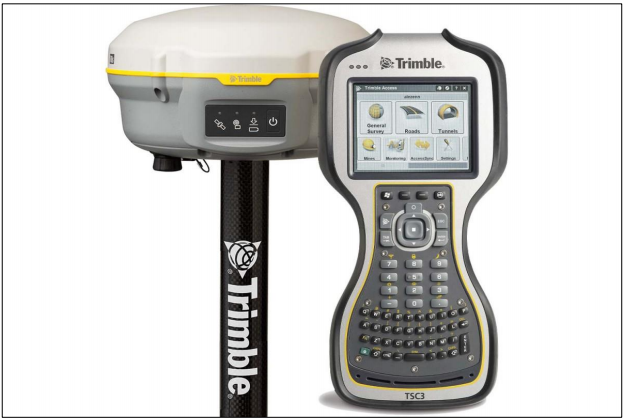
\includegraphics[scale=1]{spytnik.png}}
        \caption{ГНСС приемник Trimble R8s GNSS}
        \label{fig:image}
    \end{figure}
    
\end{newpage}

\begin{newpage}

    \begin{center}
        \begin{flushleft}
            Таблица 1 – Технические характеристики ГНСС приемника Trimble R8s
        \end{flushleft}
     
        \begin{tabular}{ | p{200pt} | p{260pt} | }
            \hline
            Количество каналов & 440\\
            \hline
            NAVSTAR GPS: & L1, L2C, L2E, L5\\
            \hline
            ГЛОНАСС: & L1C/A, L1P, L2C/A, L2P, L3\\
            \hline
            BeiDou: & B1, B2\\
            \hline
            Galileo & E1, E5A, E5B\\
            \hline
            SBAS & есть\\
            \hline
            DIFF & -\\
            \hline
            СКО Статика в плане & 3.0 мм + 0.5 мм/км\\
            \hline
            СКО Статика по высоте & 5.0 мм + 0.5 мм/км\\
            \hline
            СКО Статика быстрая в плане & 3.0 мм + 0.5 мм/км\\
            \hline
            СКО Статика быстрая по высоте & 5.0 мм + 0.5 мм/км\\
            \hline
            СКО PPK в плане & 8.0 мм + 1.0 мм/км\\
            \hline
            СКО PPK по высоте & 15.0 мм + 1.0 мм/км\\
            \hline
            СКО RTK в плане & 8.0 мм + 1.0 мм/км\\
            \hline
            СКО RTK по высоте & 15.0 мм + 1.0 мм/км\\
            \hline
            СКО DGPS в плане & 0.25 м + 1.0 мм/км\\
            \hline
            СКО DGPS по высоте & 0.50 м + 1.0 мм/км\\
            \hline
            Время инициализации, сек & <8 сек.\\
            \hline
            Частота позиционирования, Гц  & 1, 2, 5, 10, 20\\
            \hline
            Надежность инициализации & >99.9\%\\
            \hline
            Кол-во интерфейсов RS232 & 2\\
            \hline
            Bluetooth 2.0 & есть\\
            \hline
            Встроенный модем GSM/GPRS & опция\\
            \hline
            Встроенный УКВ модем  & опция (Rx, Tx)\\
            \hline
            Мощность передачи, Вт & 0.5\\
            \hline
            Частотный диапазон, МГц & 403-473\\
            \hline
            Возможность подключения внешних GSM и УКВ модемов & есть\\
            \hline
            Форматы поправок & RTCM 2.1, RTCM 2.3, RTCM 3.0, RTCM 3.1, CMR+, CMRx\\
            \hline
            Вывод сообщений формата & опция (NMEA, GSOF, RT17 и RT27,  поддержка BINEX и сглаженной несущей)\\
            \hline
            Поддерживаемые эфирные протоколы & Trimble, Pacific Crest, SATEL\\
            \hline
            Форматы записи спутниковых измерений & t02\\
            \hline
        \end{tabular}
    \end{center}
    
\end{newpage}

\begin{newpage}

    \begin{center}
        \begin{flushleft}
            Продолжение таблицы 1.
        \end{flushleft}
        \begin{tabular}{ | p{200pt} | p{260pt} | }
            \hline
            Встроенная память  & 56Мб\\
            \hline
            Размер (d, h), мм & 190 x 104\\
            \hline
             Материал корпуса & пластик\\
            \hline
            Масса приемника, кг & 1.52\\
            \hline
            Температура рабочая & От -40° до +65° C\\
            \hline
            Температура хранения & От -40° до +75° C\\
            \hline
            Пыле- и влагозащищённость & IP67\\
            \hline
            Ударостойкость & 2.0\\
            \hline
            Влажность & 100\%, с конденсацией\\
            \hline
            Погружение в воду на глубину & до 1.0 м\\
            \hline
            Потребляемая мощность & 3.2 Вт\\
            \hline
            Тип батареи & Li-Ion\\
            \hline
            Ёмкость одной батареи, мАч & 2800\\
            \hline
            Количество батарей в приемнике & 1\\
            \hline
            Количество батарей в штатном комплекте & 2\\
            \hline
            Время работы в Статике, в часах & 5.0\\
            \hline
            Время работы в RTK, в часах & 5.0\\
            \hline
            Вход внешнего питания, В & 11-28\\
            \hline
            Веб-интерфейс & есть\\
            \hline
            Измерение фазы несущей частоты с низким уровнем шума & есть\\
            \hline
            Технология подавления многолучёвост & есть\\
            \hline
            
        \end{tabular}
    \end{center}

\end{newpage}

\begin{newpage}

    \begin{center}
        \textbf{Тахеометр Trimble М3 DR 3”}
    \end{center}
    
    \begin{figure}[h]
        \center{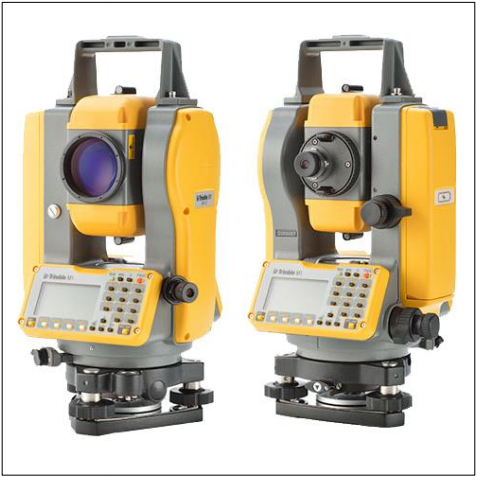
\includegraphics[scale=1]{taxeometr.png}}
        \caption{Тахеометр Trimble М3 DR 3”}
        \label{fig:image}
    \end{figure}
    
    \begin{center}
        \begin{flushleft}
            Таблица 2 – Технические характеристики тахеометра Trimble М3 DR 3”
        \end{flushleft}
     
        \begin{tabular}{ | p{200pt} | p{260pt} | }
            \hline
            Точность угловых измерений & 3"\\
            \hline
            Компенсатор &Двухосевой\\
            \hline
            Тип компенсатора & Жидкостно-электрический детектор\\
            \hline
            Диапазон компенсации & ±3'\\
            \hline
            Увеличение зрительной трубы & 33x\\
            \hline
            Минимальное фокусное расстояние  & 1,5м\\
            \hline
            Лазерный визир & Да\\
            \hline
            Дальность измерений по призме & до 5 000 м\\
            \hline
            Дальность измерений DR (без отражателя)  & до 300 м\\
            \hline
            Точность измерения расстояний & ±(3 мм + 2 ppm)\\
            \hline
            В точном безотражательном режиме & ±(3 мм + 2 ppm)\\
            \hline
            Трегер & Съемный, 3-штырьковый, типа Wild\\
            \hline
        \end{tabular}
    \end{center}

\end{newpage}

\begin{newpage}
    
    \begin{center}
        \begin{flushleft}
            Продолжение таблицы 2.
        \end{flushleft}
     
        \begin{tabular}{ | p{200pt} | p{260pt} | }
            \hline
            Точность угловых измерений & 3"\\
            \hline
            Компенсатор &Двухосевой\\
            \hline
            Тип компенсатора & Жидкостно-электрический детектор\\
            \hline
            Диапазон компенсации & ±3'\\
            \hline
            Увеличение зрительной трубы & 33x\\
            \hline
            Минимальное фокусное расстояние  & 1,5м\\
            \hline
            Лазерный визир & Да\\
            \hline
            Дальность измерений по призме & до 5 000 м\\
            \hline
            Дальность измерений DR (без отражателя)  & до 300 м\\
            \hline
            Точность измерения расстояний & ±(3 мм + 2 ppm)\\
            \hline
            В точном безотражательном режиме & ±(3 мм + 2 ppm)\\
            \hline
            Трегер & Съемный, 3-штырьковый, типа Wild\\
            \hline
        \end{tabular}
    \end{center}

\end{newpage}

\begin{newpage}
    
    \begin{center}
        \textbf{Теодолит электронный DT2A}
    \end{center}
    
    \par Теодолит электронный DT2A – это простой в управлении высокоточный  инструмент. Он к минимуму сводит ошибки оператора в процессе работы и поэтому в первую очередь на него следует обратить внимание начинающим специалистам. Теодолит имеет двустороннюю панель управления и компенсатор с диапазоном ±3´. Угловая точность теодолита 2".

    \begin{figure}[h]
        \center{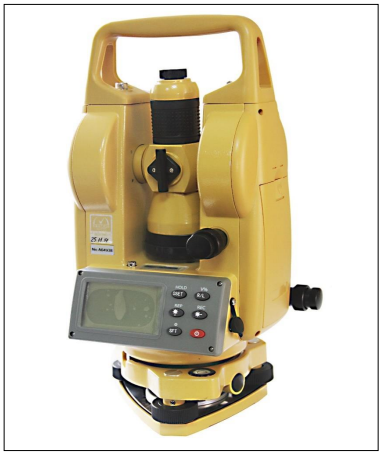
\includegraphics[scale=1]{teodolit.png}}
        \caption{Теодолит электронный DT2A}
        \label{fig:image}
    \end{figure}
    
    \begin{center}
        \begin{flushleft}
            Таблица 3 – Технические характеристики электронного теодолита DT2A
        \end{flushleft}
        
        \begin{tabular}{ | p{200pt} | p{260pt} | }
            \hline
            Наименование & Характеристики\\
            \hline
            Точность угловых измерений  & 2"\\
            \hline
            Дискретность отсчета & 1" / 5"\\
            \hline
            Точность компенсации & ±3'\\
            \hline
            Увеличение зрительной трубы & 30Х\\
            \hline
            Диаметр объектива  & 45мм\\
            \hline
            Изображение & прямое\\
            \hline
            Поле зрения & до 1º 30´\\
            \hline
            Трегер & съемный, типа Wild\\
            \hline
            Отвес & лазерный\\
            \hline
        \end{tabular}
    \end{center}
    
\end{newpage}

\begin{newpage}
        
    \begin{center}
        \begin{flushleft}
            Продолжение таблицы 3.
        \end{flushleft}
        
        \begin{tabular}{ | p{200pt} | p{260pt} | }
            \hline
            Панель управления & двусторонняя\\
            \hline
            Дисплей & с двух сторон LCD\\
            \hline
            Передача данный на компьютер & кабель RS232С (в комплект не входит)\\
            \hline
            Питание & 4хАА\\
            \hline
            Время работы от одной батареи & около 20 часов\\
            \hline
            Рабочая температура & -20ºС - +50ºС\\
            \hline
            Вес & 4,7 кг\\
            \hline
            Минимальное фокусное расстояние & 1,3 м\\
            \hline
            Длина телескопа & 156 мм\\
            \hline
            Датчик наклона & есть\\
            \hline
            Диапазон & ±3´\\
            \hline
        \end{tabular}
    \end{center}
    
\end{newpage}

\begin{newpage}
        
        \begin{center}
            \textbf{Цифровой нивелир DL-202}
        \end{center}
        
        \begin{figure}[h]
            \center{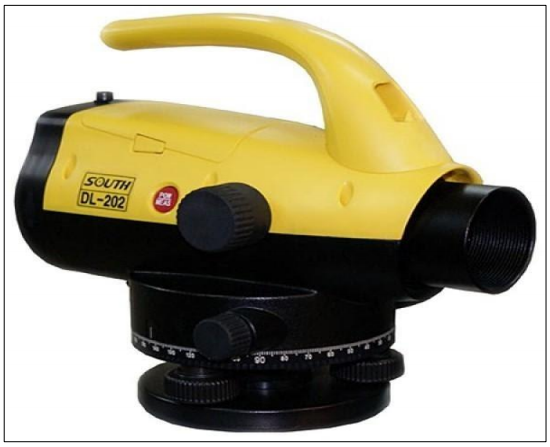
\includegraphics[scale=1]{nivelir.png}}
            \caption{Цифровой нивелир DL-202}
            \label{fig:image}
        \end{figure}
        
        \begin{center}
            \begin{flushleft}
                Таблица 4 – Технические характеристики цифрового нивелира DL-202
            \end{flushleft}
            
            \begin{tabular}{ | p{200pt} | l | }
                \hline
                 & электронное измерение на фиберглассовую\\
                Точность нивелирования (CКО на 1 км двойного хода) & рейку 1.5 мм\\
                \cline{2-2}
                 & оптическое измерение 2.0 мм\\
                \hline
                Точность измерения дальности & 10 мм\\
                \hline
                Диапазон измерения & от 1,5 до 100 м\\
                \hline
                Время измерения & 3 сек.\\
                \hline
                 & изображение прямое\\
                \cline{2-2}
                Зрительная труба & увеличение 32Х\\
                \cline{2-2}
                 & поле зрения 1020′\\
                \hline
                Компенсатор & тип маятниковый, с магнитным демпфером\\
                \hline
                 & диапазон ±12′\\
                 \hline
                 & точность способность 0,5″/1′\\
                \hline
                Встроенная память & 16 МБ\\
                \hline
                Точность круглого пузырькового уровня & 8′/ 2 мм\\
                \hline
            \end{tabular}
    \end{center}
        
\end{newpage}

\begin{newpage}

        \begin{center}
            \begin{flushleft}
                Продолжение таблицы 4.
            \end{flushleft}
            \begin{tabular}{ | p{200pt} | p{260pt} | }
                \hline
                Дисплей & LCD, 128×32 dpi\\
                \hline
                Защита & IP54\\
                \hline
                Рабочая температура & —20…50$^\circ$C\\
                \hline
                Время работы от встроенных батарей & 15 часов\\
                \hline
                Габариты & 270х210х180 мм\\
                \hline
                Вес & 2,5 кг\\
                \hline
            \end{tabular}
    \end{center}
        
\end{newpage}

\begin{newpage}

    \begin{flushright}
        Приложение Б. Поверки электронного нивелира DL−202
    \end{flushright}
    
    \large{
        \par\textbf{1. Поверка круглого уровня}
        \par\textbf{Выполнение:} Вращая подъемные винты подставки нивелира, приводят пузырек круглого уровня в нуль-пункт. Затем поворачивают уровень вместе со зрительной трубой нивелира по азимуту на 180$^\circ$. Если при этом пузырек останется в центре ампулы, то условие выполнено. В противном случае, действуя исправительными винтами уровня, перемещают пузырек на половину дуги отклонения его от нуль-пункта в направлении к центру ампулы, а на вторую половину отклонения — при помощи подъемных винтов. После этого вновь производят поверку. Так поступают до тех пор, пока условие не будет выполнено.
        \par\textbf{Результат:} Поверка выполняется.\\
    
        \par\textbf{2. Вертикальная нить сетки должна совпадать с отвесом (быть параллельна вертикальной оси вращения нивелира).}
        \par\textbf{Выполнение:} Для выполнения этой поверки в защищенном от ветра месте подвешивают на тонком шнуре тяжелый отвес. На расстоянии 20—25 м от отвеса устанавливают поверяемый нивелир и приводят его в рабочее положение (при помощи элевационного винта совмещают видимые в поле зрения трубы концы пузырька цилиндрического уровня). Затем один конец вертикальной нити сетки совмещают с отвесом. Если другой конец этой нити отойдет от отвеса более, чем на 0,5 мм, то исправляют установку сетки в зрительной трубе. Для этого снимают окулярную часть зрительной трубы и отпускают винты, крепящие оправу пластинки с сеткой нитей к корпусу трубы. Затем, перемещая пластинку, устанавливают сетку в соответствующее положение, закрепляют винты и присоединяют окуляр, и вновь повторяют эту поверку.
        \par\textbf{Результат:} Поверка выполняется.\\
    
        \par\textbf{3. Ось цилиндрического уровня должна быть параллельна визирной оси зрительной трубы.}
        \par\textbf{Выполнение:} Проверка этих условий выполняется двойным нивелированием пары точек способом "из середины" и "вперед"(рис.33). Для этого закрепляют неподвижно две нивелирные рейки на расстоянии 60-90 м, а нивелир устанавливают между ними на середину с погрешностью 1 м. Расстояния до реек измеряют нитяным дальномером. Определяют превышение между рейками при двух горизонтах прибора, как разность отсчетов на заднюю и переднюю рейки. Превышение, полученное при одном горизонте прибора, не должно отличаться от превышения, полученного при втором горизонте прибора, не более 3 мм. Затем выбирают вторую станцию на расстоянии предела фокусирования (2...3 м) от одной из реек и берут по ней отсчет. Используя этот отсчет и превышение, полученное на первой станции вычисляют отсчет по дальней рейке.
        \par\textbf{Результат:} Поверка выполняется.\\
    }

\end{newpage}

\begin{newpage}

    \begin{flushright}
        Приложение В. Поверки электронного теодолита DT-2A
    \end{flushright}
    \large{
        \par\textbf{1. Поверка цилиндрического уровня}
        \par\textbf{Главное условие:} Ось цилиндрического уровня должна быть перпендикулярна вертикальной оси инструмента.
        \par\textbf{Выполнение:} Установите инструмент так, чтобы ось
        цилиндрического уровня была параллельна двум установочным
        винтам. С помощью этих винтов загоните пузырь уровня в центр
        колбы уровня. Поверните инструмент на 180˚ вертикальной оси и проверьте
        движение пузыря цилиндрического уровня. Если пузырь переместился, следует выполнить юстировку.
        \par\textbf{Вывод:} Поверка выполняется.
        \par\textbf{Юстировка:} Отрегулируйте положение пузырька уровня спомощью шпильки из набора аксессуаров к инструменту, чтобы он переместился к центру колбы на половину своего отклонения. Откорректируйте оставшуюся половину отклонения с помощью установочных винтов. Поверните инструмент на 180˚ вертикальной оси и проверьте движение пузыря цилиндрического уровня. Если пузырь переместился, следует повторить регулировку.\\
    
        \par\textbf{2. Поверка круглого уровня}
        \par\textbf{Главное условие:} Ось круглого уровня должна быть параллельна оси вращения инструмента.
        \par\textbf{Выполнение:} До начала данной поверки должна
        быть выполнена юстировка цилиндрического уровня (если в этом
        есть необходимость). Если пузырёк круглого уровня находится в
        нуль-пункте после приведения в центр пузырька цилиндрического уровня, то дальнейшая юстировка не требуется. В противном случае необходима юстировка.
        \par\textbf{Вывод:} Поверка выполняется.
        \par\textbf{Юстировка:} Действуя юстировочной шпилькой, повернуть
        юстировочные винты, пока пузырёк круглого уровня не переместится в центр. Во избежание разрыва, нельзя перетягивать юстировочные винты.\\
    
        \par\textbf{3. Поверка сетки нитей телескопа}
        \par\textbf{Главное условие:} Вертикальные нити сетки нитей телескопа должны быть перпендикулярны горизонтальной оси инструмента.
        \par\textbf{Выполнение:} Тщательно отгоризонтируйте инструмент на треггере. Наведите сетку нитей на хорошо видимую точку А с дистанции не менее 50 м. Качните телескоп по вертикали и проверьте скользит ли точка А вдоль всей вертикальной нити. Если точка А скользит вдоль всей вертикальной нити, то вертикальные нити сетки нитей телескопа перпендикулярны горизонтальной оси инструмента. Юстировка в этом случае не требуется. Если точка А при качении оптической трубы вдоль вертикали отклоняется от вертикальной нити сетки нитей, то в этом случае юстировка требуется.
        \par\textbf{Вывод:} Поверка выполняется.
        \par\textbf{Юстировка:} Отвинтите крышку покрывающую 4 регулировочных винта сетки нитей поворачивая крышку против часовой стрелки. Ослабте эти винты отверткой из набора аксессуаров, считая при этом число оборотов отвёртки. Совместите вертикальную нить сетки нитей с точкой А и затяните регулировочные винты тем же количеством оборотов отвёртки. Проведите проверку до тех пор пока точка А не будет скользить по всей длине вертикальной нити сетки нити.\\
    
        \par\textbf{4. Коллимация инструмента}
        \par\textbf{Главное условие:} Визирная ось телескопа должна быть перпендикулярна горизонтальной оси инструмента.
        \par\textbf{Выполнение:} Установите инструмент между точками А и В в пределах их прямой видимости на равном расстоянии 50 – 60м от каждой из них. Тщательно отгоризонтируйте инструмент на триггере по цилиндрическому уровню. Наведитесь на А. Ослабьте затяжной винт вертикальной наводки и поверните трубу на 180˚ вокруг горизонтальной оси инструмента т.о. чтобы труба показывала в противоположную сторону. Наведитесь на точку В и закрепите затяжной винт вертикальной наводки. Ослабте затяжной винт горизонтальной наводки и поверните трубу на 180˚ вокруг вертикальной оси инструмента т.о. чтобы труба показывала в противоположную сторону. Наведитесь на точку А и закрепите затяжной винт горизонтальной наводки. Ослабьте затяжной винт вертикальной наводки и поверните трубу на 180˚ вокруг горизонтальной оси инструмента. Перекрестие сетки нитей телескопа (точка С) должно совпасть с точкой В. Если точка С не совпадает с точкой В то требуется регулировка состоящая из следующих процедур.
        \par\textbf{Вывод:} Поверка выполняется.
        \par\textbf{Юстировка:} Отвинтите крышку покрывающую 4 регулировочные винты сетки нитей. Регулировочных винта сетки нитей поворачивая крышку против часовой стрелки. Определите точку D между В и С т.о. чтобы расстояние CD равнялось ¼ расстояния ВС. (несовпадение ВС в 4 раза больше реальной ошибки за коллимацию из-за того что телескоп при проверке поворачивался 2 раза. Поворачивая регулировочные воротки в верхней, нижней, левой и правой части окуляра передвиньте вертикальную нить сетки нитей т.о. чтобы она совпадала с точкой D. По окончании регулировки повторите процедуру проверки. Если точки В и С совпадают, то дальнейшей регулировки не требуется. В противном случае повторите регулировку.\\
    
        \par\textbf{5. Поверка лазерного отвеса.}
        \par\textbf{Главное условие:} Вертикальная ось теодолита должна находиться над точкой центрирования когда лазерный визир будет попадать на точку центрирования.
        \par\textbf{Выполнение:} Установите инструмент на штатив на высоту около 1.5м и отгоризонтируйте его. Включите лазерный отвес и заметьте первоначальное расположение лазерного визира на земле. Поверните инструмент на 180˚ вокруг вертикальной оси и проверьте точку на земле. Если первоначальная точка центрирования остаётся в пределах 1мм от первоначального положения визира регулировки не требуется. В противном случае требуется регулировка состоящая из следующих процедур.
        \par\textbf{Вывод:} Поверка выполняется.
        \par\textbf{Юстировка:} Отвинтите крышку регулировочной части окуляра отвеса. Под ней находятся 4 регулировочных винта воротков. Отрегулируйте положение воротков окуляра с помощью шпильки из набора аксессуаров т. о. чтобы передвинуть первоначальную точку центрирования к лазерному визиру на ½ величины её от5 клонения от визира. Поверните инструмент на 180˚ вокруг вертикальной оси и проверьте точку на земле. Если первоначальная точка центрирования остаётся менее 1мм от первоначального положения визира регулировки не требуется. В противном случае требуется повторение регулировки.\\
    }

\end{newpage}

\begin{newpage}

    \begin{flushright}
        Приложение Г. Абрисы пунктов
    \end{flushright}
    
    \begin{center}
            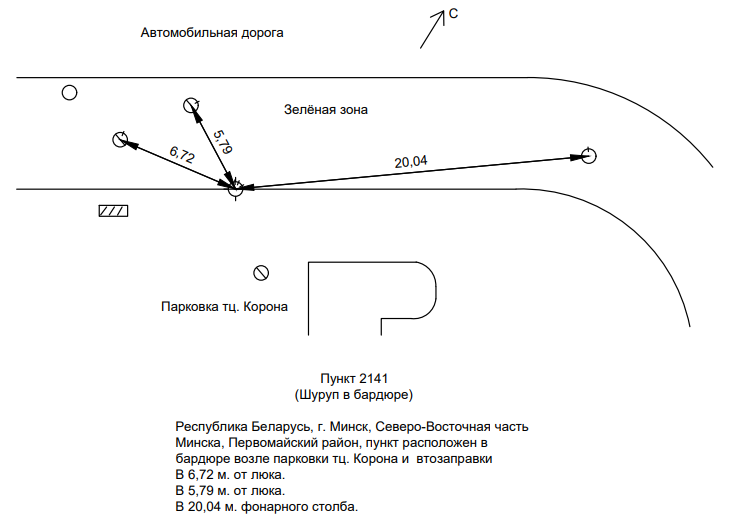
\includegraphics[scale=1.2]{abrisy/Абрис 2141.png}
            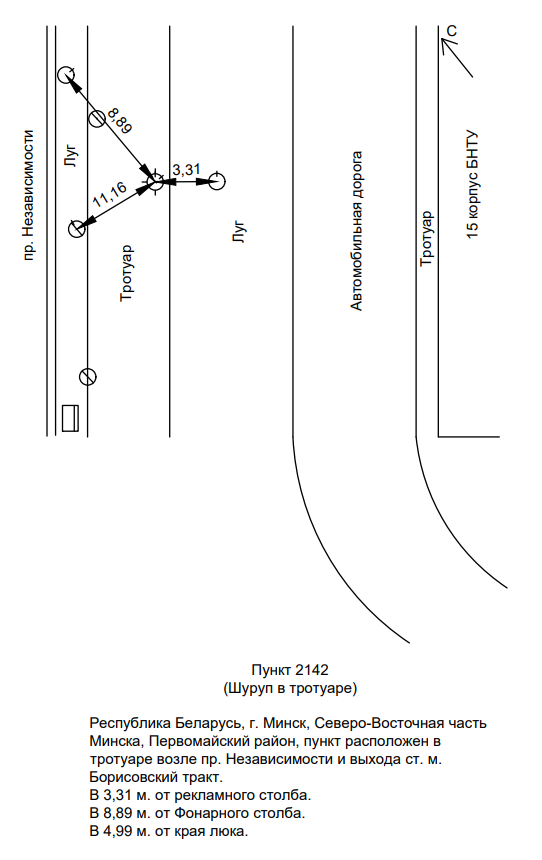
\includegraphics[scale=1.2]{abrisy/Абрис 2142.png}
            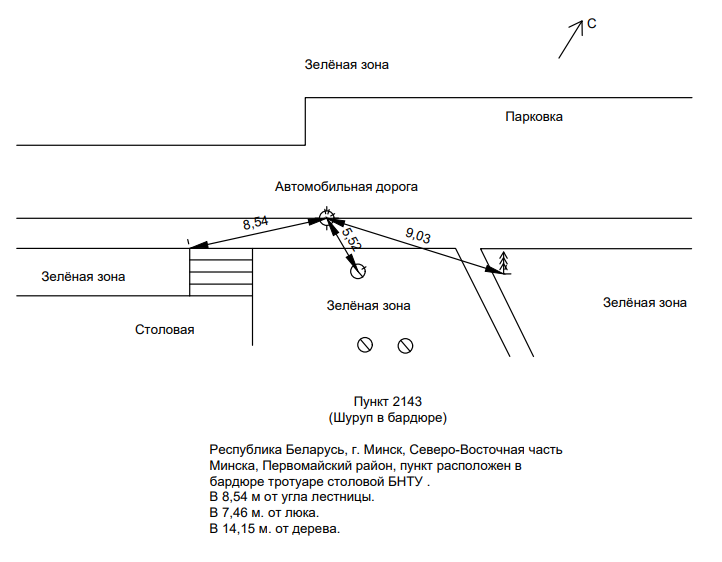
\includegraphics[scale=1.2]{abrisy/Абрис 2143.png}
            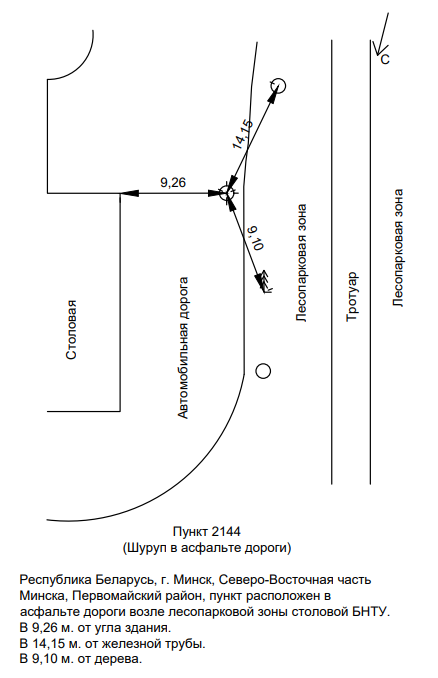
\includegraphics[scale=1.2]{abrisy/Абрис 2144.png}
            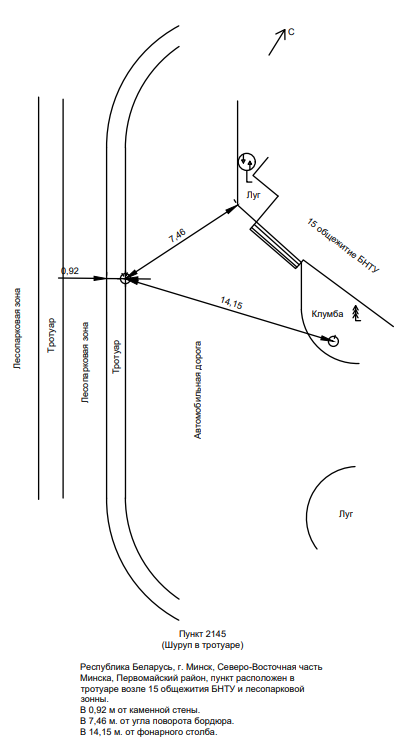
\includegraphics[scale=1.2]{abrisy/Абрис 2145.png}
    \end{center}

\end{newpage}


\begin{newpage}

    \begin{flushright}
        Приложение Д. Ведомость круговых приёмов
    \end{flushright}
    
    \begin{center}
        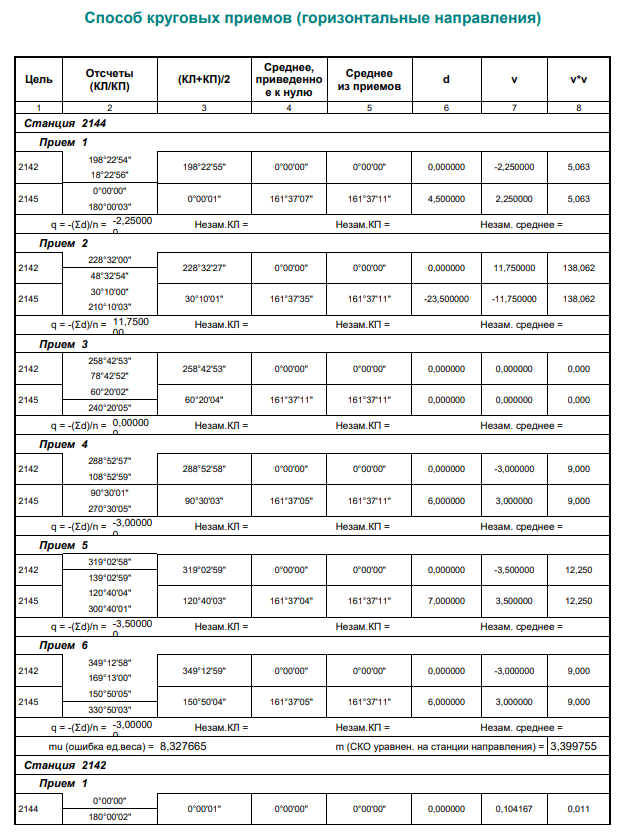
\includegraphics[scale=1.36]{vedomosty/скп1.png}
        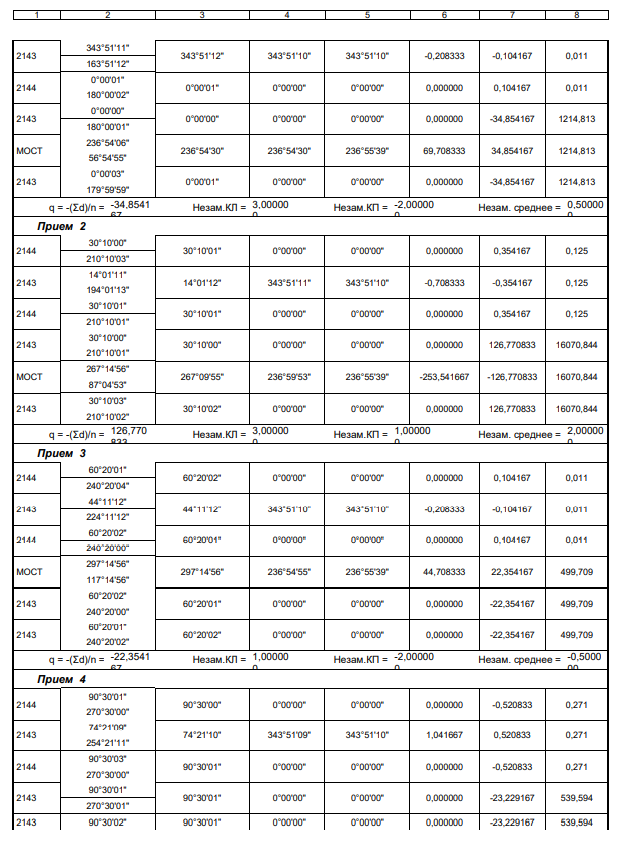
\includegraphics[scale=1.4]{vedomosty/скп2.png}
        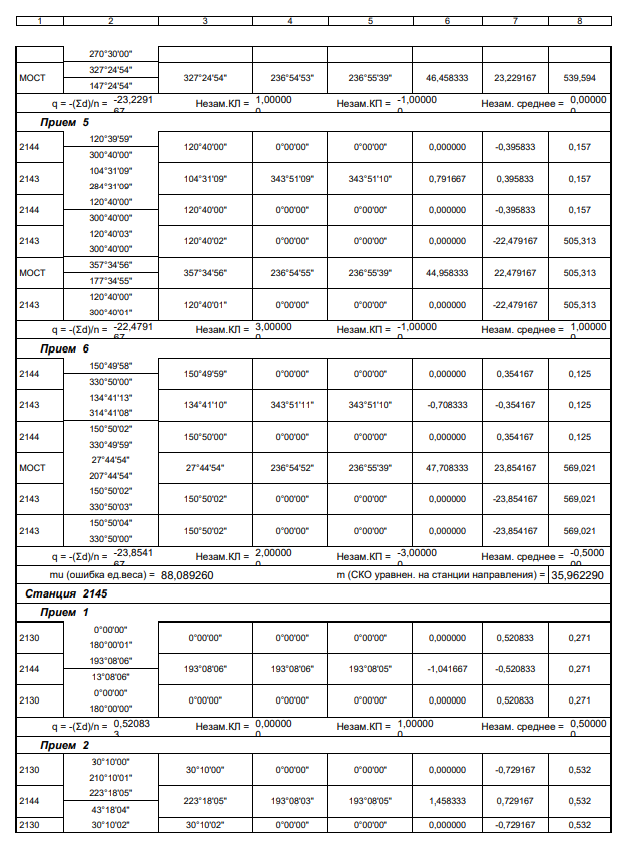
\includegraphics[scale=1.4]{vedomosty/скп3.png}
        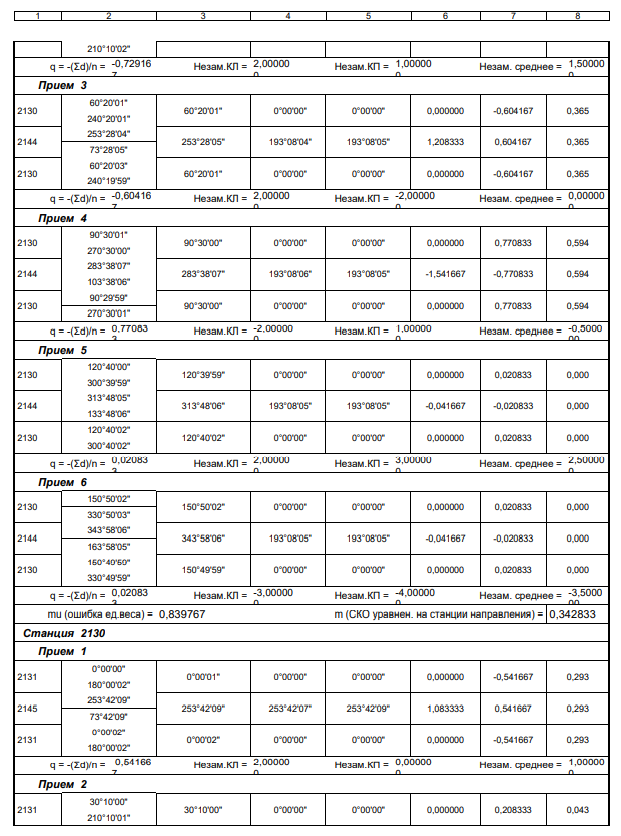
\includegraphics[scale=1.4]{vedomosty/скп4.png}
        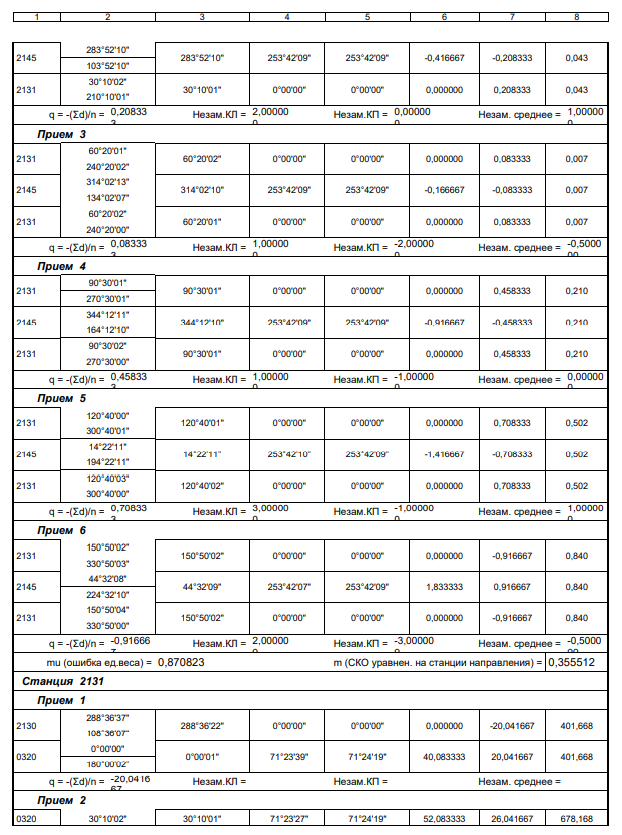
\includegraphics[scale=1.4]{vedomosty/скп5.png}
        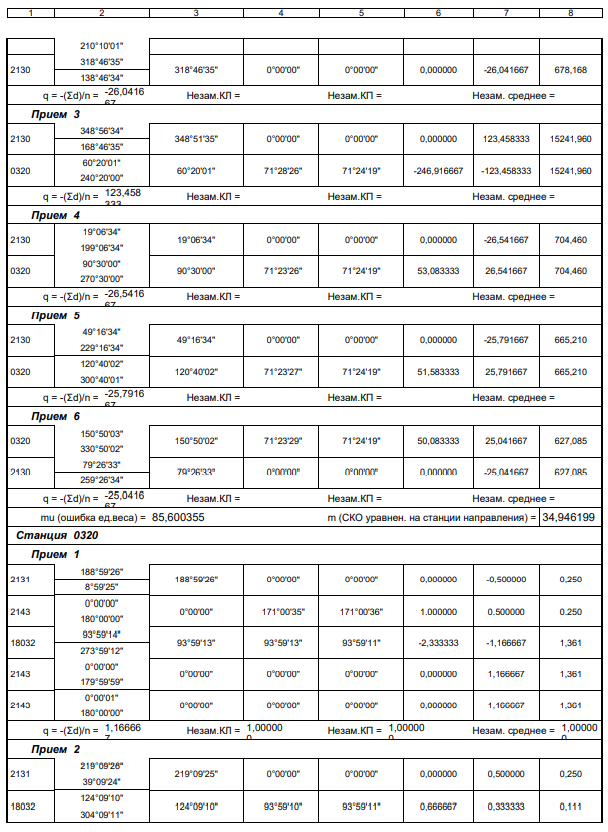
\includegraphics[scale=1.4]{vedomosty/скп6.png}
        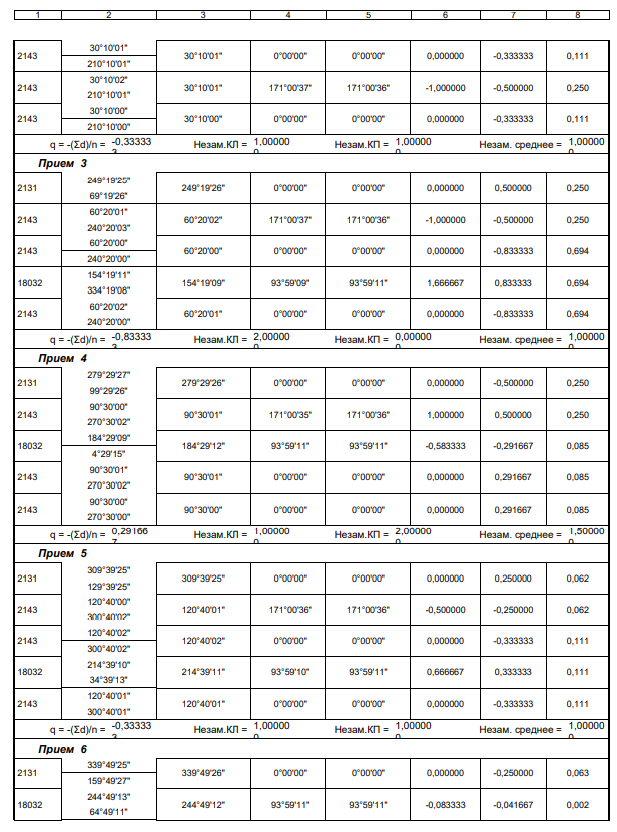
\includegraphics[scale=1.4]{vedomosty/скп7.png}
        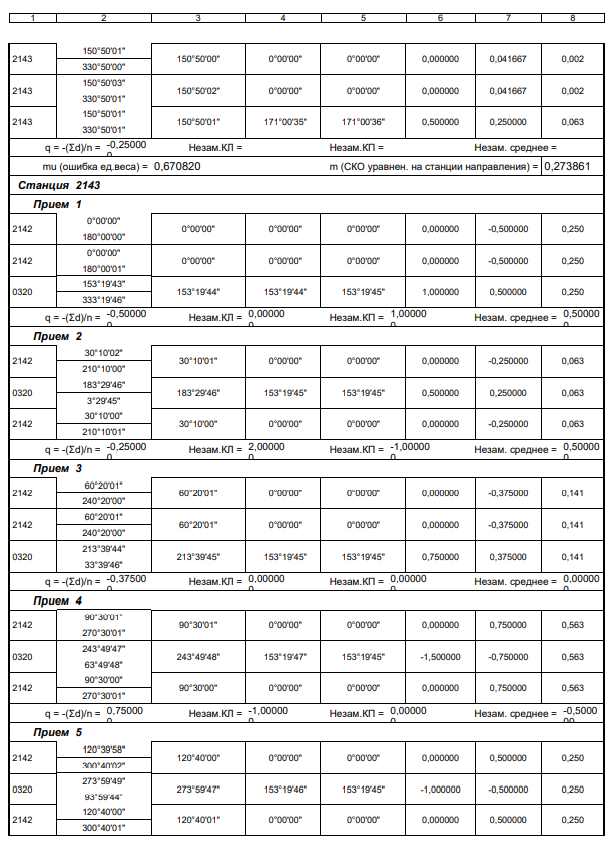
\includegraphics[scale=1.4]{vedomosty/скп8.png}
        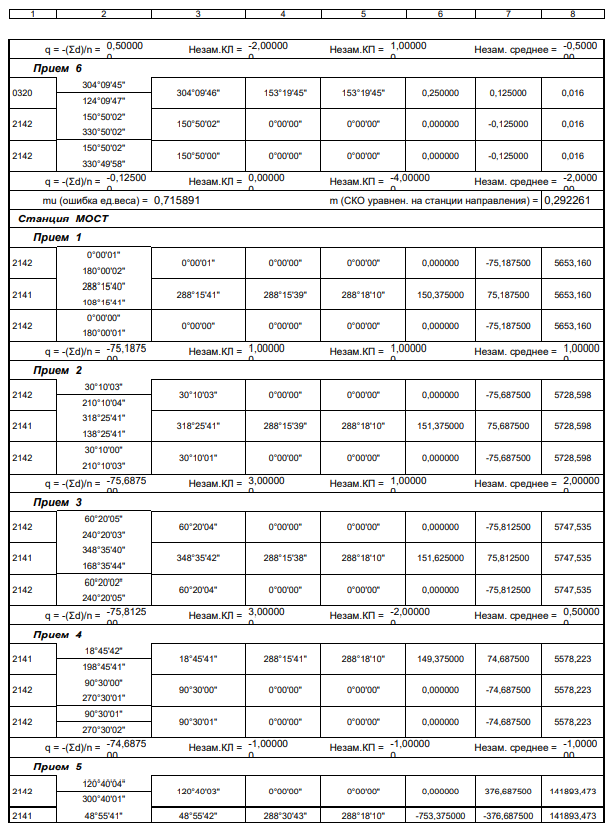
\includegraphics[scale=1.4]{vedomosty/скп9.png}
        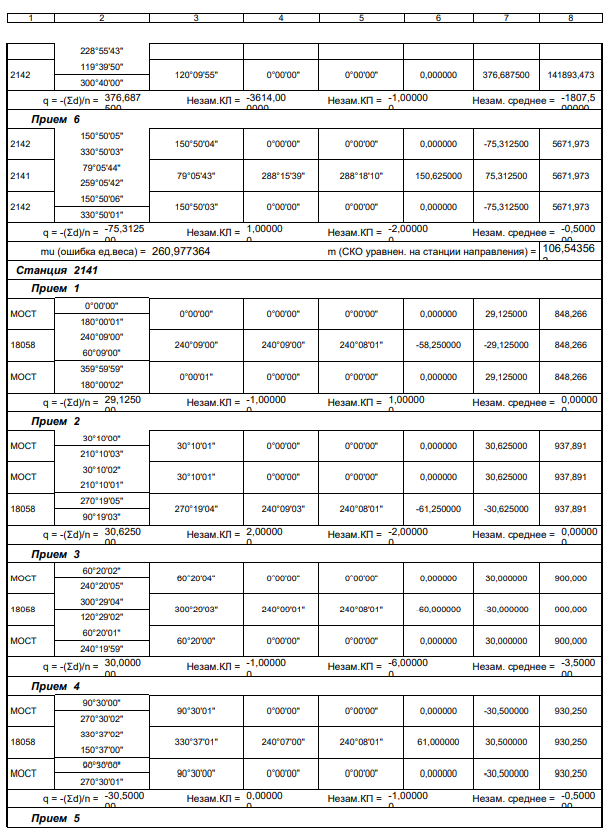
\includegraphics[scale=1.4]{vedomosty/скп10.png}
        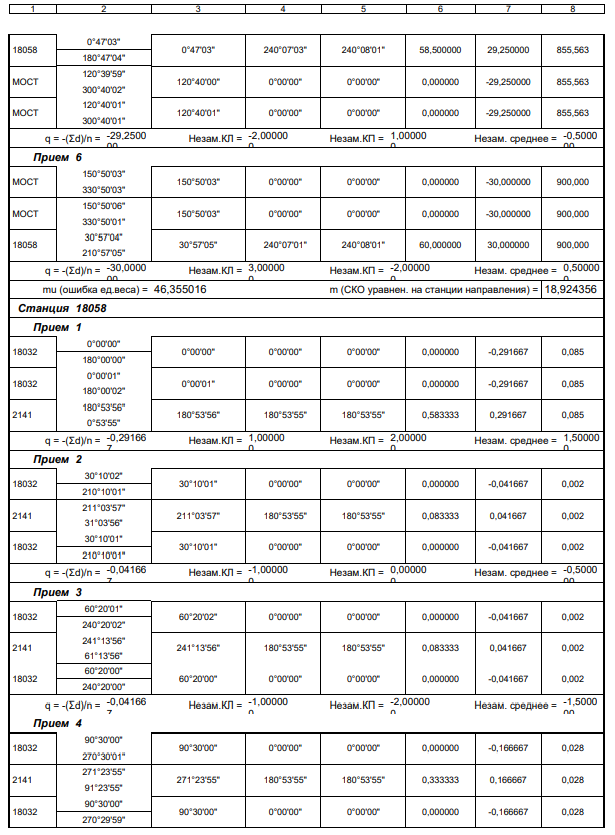
\includegraphics[scale=1.4]{vedomosty/скп11.png}
        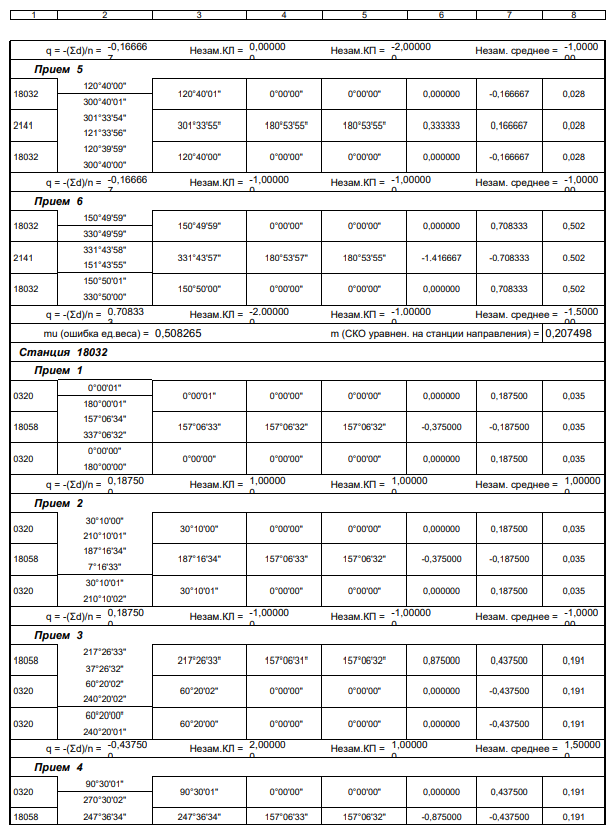
\includegraphics[scale=1.4]{vedomosty/скп12.png}
        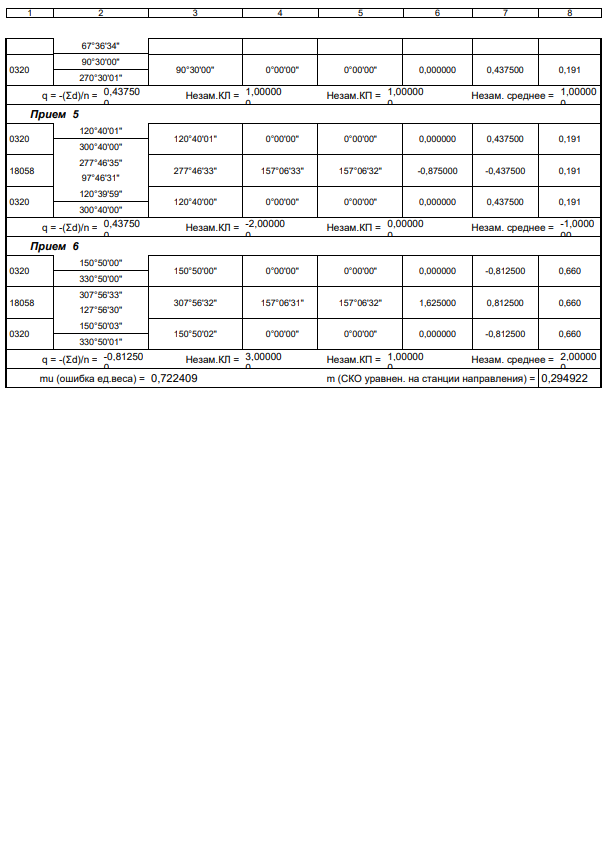
\includegraphics[scale=1.4]{vedomosty/скп13.png}
    \end{center}

\end{newpage}

\begin{newpage}

        \begin{flushright}
            Приложение Е. Журнал нивелирования III класса
        \end{flushright}
        
        \begin{center}
            \begin{flushleft}
                \: Таблица 1 - Полигон 1
            \end{flushleft}
            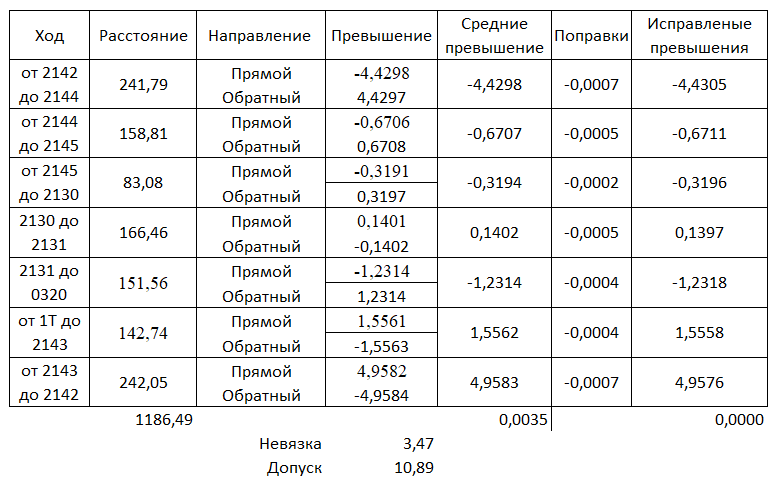
\includegraphics[scale=1.1]{N1.png}
            
            \begin{flushleft}
                \, Таблица 2 - Полигон 2
            \end{flushleft}
            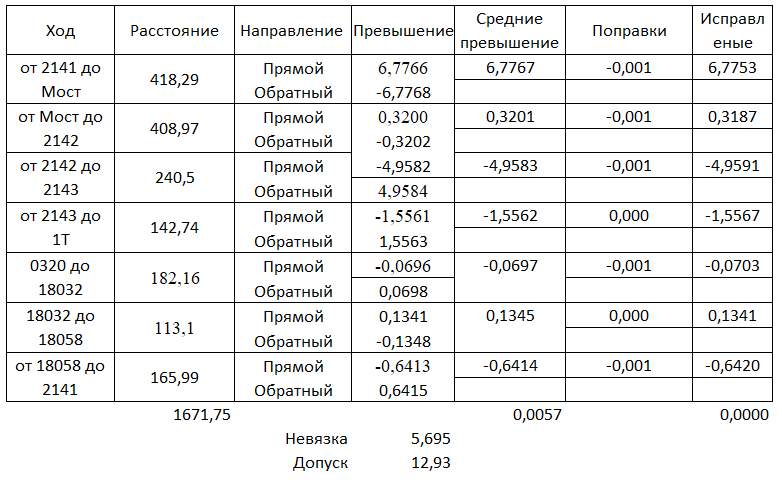
\includegraphics[scale=1.1]{N2.png}
        \end{center}

\end{newpage}

\begin{newpage}

    \begin{landscape}
        \begin{center}
            \begin{flushright}
                Приложение Ж. Ведомость оценки точности положения пунктов
            \end{flushright}
            
            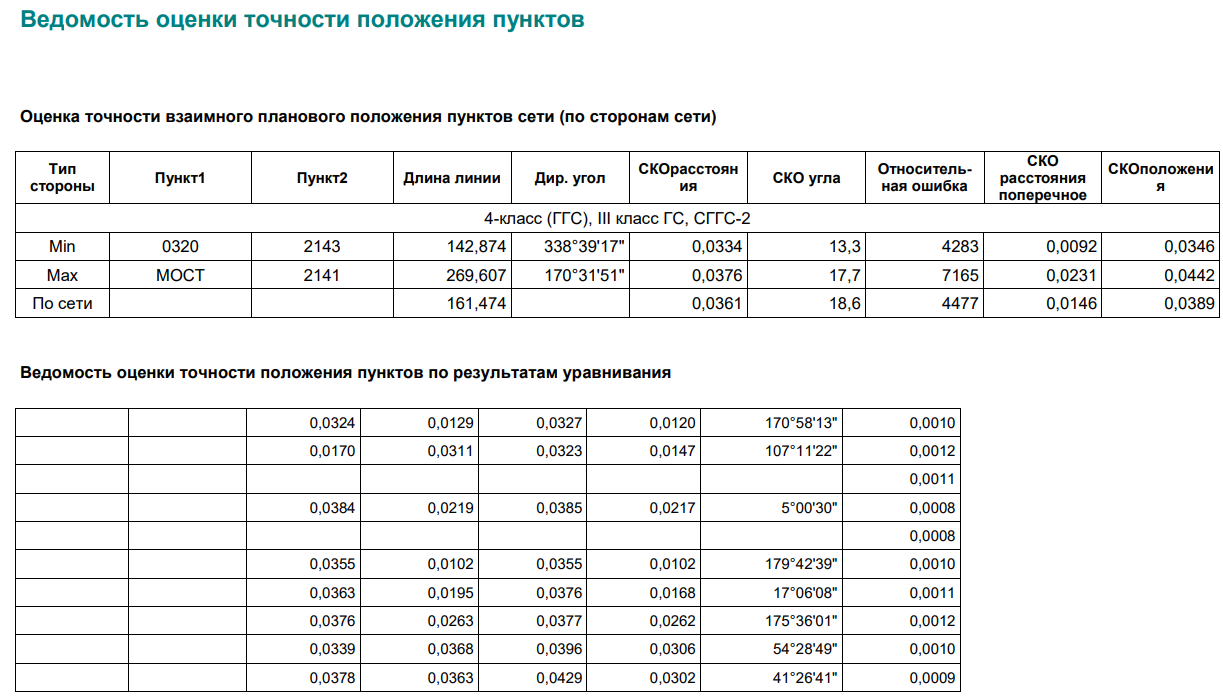
\includegraphics[scale=1]{votpp.png}
        \end{center}
    \end{landscape}

\end{newpage}

\begin{newpage}

    \begin{landscape}
        \begin{center}
            \begin{flushright}
                Приложение З. Каталог пунктов ПВО
            \end{flushright}
            
            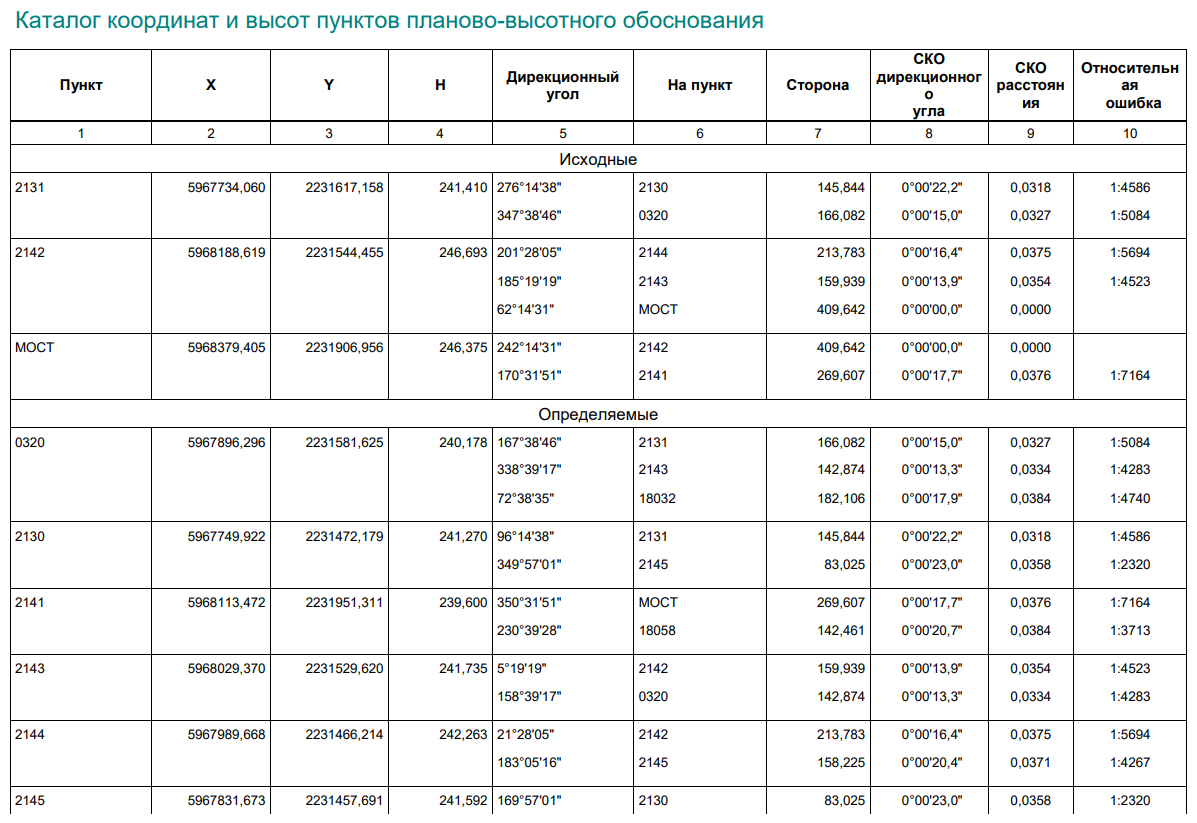
\includegraphics[scale=0.93]{kkivpp-vo.png}
        \end{center}
    \end{landscape}

\end{newpage}

\begin{newpage}

        \begin{center}
            \begin{flushright}
                Приложение И. Схема сети полигонометрии
            \end{flushright}
            ~\\
            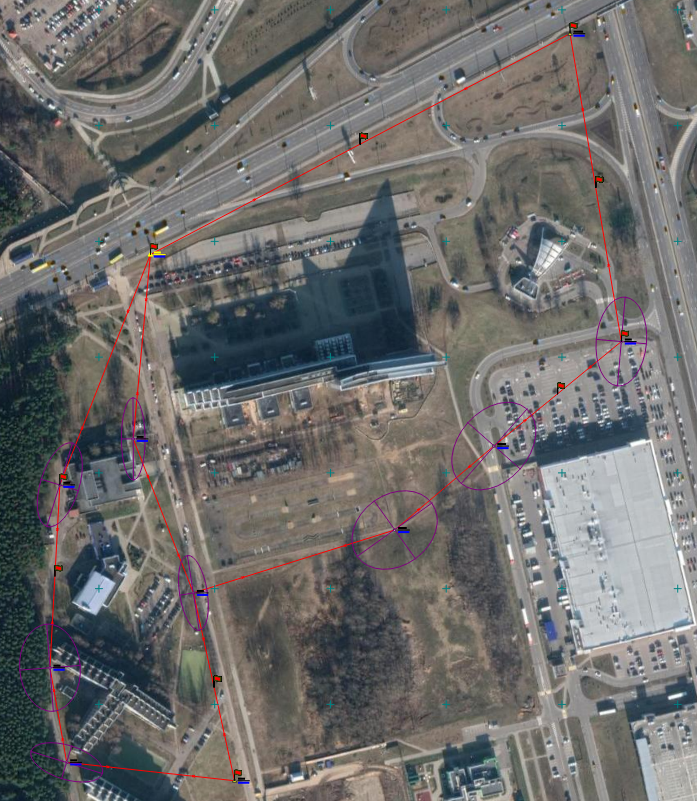
\includegraphics[scale=1]{shema.png}
        \end{center}

\end{newpage}

\end{document}
